\chapter{Test utilisateurs}
	Le test utilisateur est une étape indispensable pour valider les
	théories développées durant le travail de recherche et conception.
	Ces tests auront pour but de valider deux aspects du framework : Ses
	performances lors de la peinture d'image gigapixel, et la qualité
	de son anti-aliasing. 

	\section{Procédure}
		Le but de la procédure est d'arriver à obtenir de l'artiste une
		information fiable sur la performance du framework et la qualité du rendu. 
		Cela n'est pas une chose évidente puisque l'artiste ne fait habituellement
		pas la différence entre l'interface utilisateur et le framework utilisé pour
		le rendu. 

		\subsection{Premiers tests}
		En effet, les premiers tests furent réalisés avec une interface graphique fort
		austère et différente des logiciels que les artistes avaient l'habitude d'utiliser.
		La plupart de leurs critiques étaient centrées sur l'interface utilisateur, et
		leur évaluation des performances semblaient affectée par la frustration générée
		par l'interface graphique.

		Nous avons donc décidé d'améliorer l'interface en répondant aux principales critiques
		des utilisateurs:
		\begin{itemize}
			\item nécessité d'avoir un outil permettant de sélectionner une couleur à l'écran.
			\item nécessité d'avoir des raccourcis clavier similaires à \emph{Adobe Photoshop}
			\item nécessité d'avoir une visualisation de la taille de la brush autour du curseur.
		\end{itemize}

		\begin{figure}[ht]
			\centering
			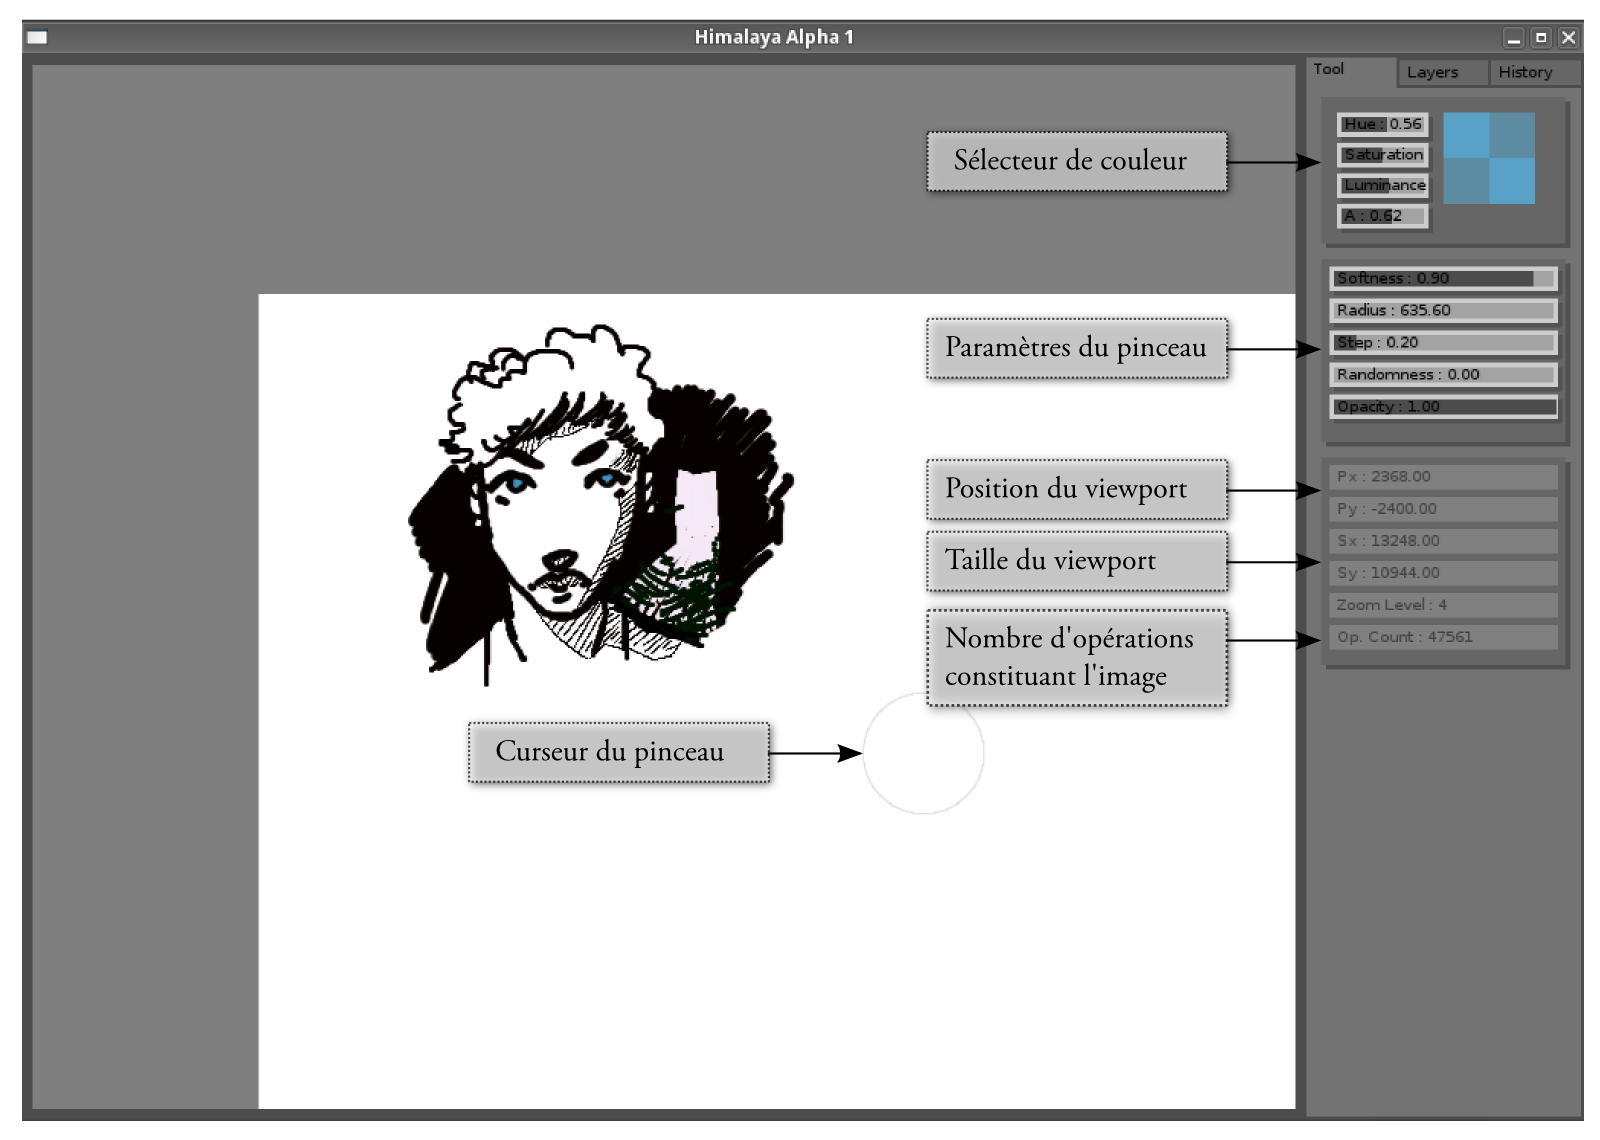
\includegraphics[width=\textwidth]{images/screenshot} 
			\caption{Screenshot de l'application utilisée pour les tests utilisateurs}
			\label{fig:screenshot}
		\end{figure}
		Ces fonctionnalités furent donc implémentées, et les tests refaits. Un screenshot de l'application
		utilisée pour les tests se trouve à la figure~\ref{fig:screenshot}, page~\pageref{fig:screenshot} 

		\subsection{Second tests}
			\subsubsection{Matériel utilisé}
			Afin de rendre comparable les évaluations de performances avec les discussions des
			précédent chapitres, les tests utilisateurs ont été réalisés sur la machine de développement.
			Il s'agit d'un ordinateur portable avec un processeur Intel à deux cores à 1.66GHz, disposant
			de 2Go de RAM, d'un écran 1024x768, avec le système d'exploitation Linux Debian Lenny.

			Les utilisateurs avaient également à leur disposition une tablette graphique Wacom Bamboo.

			\subsubsection{Première étape}
			Nous commençons par une démonstration exhaustive des fonctionnalités du programme.
			Ensuite nous expliquons le but de l'expérience; l'évaluation de la fluidité de
			l'édition, et la qualité de l'anti-aliasing --- et non pas de l'interface utilisateur.
			Nous terminons cette première étape par énoncer et expliquer toutes les étapes qui vont suivre,
			afin que l'utilisateur ne soit pas pris au dépourvu à chaque étape.

			\subsubsection{Second étape}
			Cette seconde étape constitue en une familiarisation avec l'interface. L'utilisateur
			a pour consigne de prendre le temps qu'il désire pour se familiariser avec le programme
			et tester ses fonctionnalités. 

			\subsubsection{Troisième étape}
			Les performances et la qualité du rendu peut dépendre du type de dessin réalisé. Ainsi
			nous allons explorer dans cette étape un des deux grands styles de dessin, le dessin au trait.
			Il est donc demandé à l'utilisateur de réaliser un portrait au trait, en noir et blanc de préférence.
			Il dispose pour cela d'une durée de vingt minutes. 


			L'utilisateur commence avec une feuille de dessin blanche de $800 \times 600$ Millions de pixel, au cinquième
			niveau de zoom. À ce niveau, la région visualisée a une résolution d'un demi gigapixel.

			Pendant cette étape, l'évaluateur observe, note les commentaires de l'utilisateur, et répond aux questions
			éventuelles. 

			On notera que la durée des tests, vingt minutes, est assez courte. Elle ne permet pas toujours au testeur
			de terminer son dessin. Cette durée est intentionnellement limitée pour ne pas demander trop de temps aux testeurs
			bénévoles, mais aussi pour éviter d'atteindre la limite de mémoire de la machine, étant donné que 
			le programme ne dispose pas encore de mécanisme global permettant de limiter son usage. 

			\subsubsection{Quatrième étape}
			Cette étape impose le deuxième style, la peinture à l'aplat. Il est donc demandé à l'utilisateur de
			réaliser un portrait en couleur en utilisant des techniques de peinture. 
			Il dispose pour cela d'une durée de vingt minutes. 

			L'utilisateur commence avec une feuille de dessin blanche de $800 \times 600$ Millions de pixel, au cinquième
			niveau de zoom. À ce niveau, la région visualisée a une résolution d'un demi gigapixel.

			Pendant cette étape, l'évaluateur observe, note les commentaires de l'utilisateur, et répond aux questions
			éventuelles. 

			\subsubsection{Cinquième étape}
			Cette dernière étape est conçue pour forcer les utilisateurs à utiliser toute la résolution d'une image
			gigapixel. Pour cela nous leur demandons de dessiner dans la technique de leur choix \emph{Un homme sur
			un éléphant, avec dans sa poche une puce} Le tout en respectant les échelles. 

			L'utilisateur commence avec une feuille de dessin blanche de $800 \times 600$ Millions de pixel, au sixième
			niveau de zoom. À ce niveau, la région visualisée a une résolution de deux gigapixels.

			Pendant cette étape, l'évaluateur observe, note les commentaires de l'utilisateur, et répond aux questions
			éventuelles. 

			\subsubsection{Évaluation}
			Après chaque étape nécessitant une interaction avec le programme, il est demandé à l'utilisateur de donner
			une note entre un et cinq sur les points suivants:
			\begin{itemize}
				\item Les performances lors de la peinture
				\item Les performances lors du déplacement de la région visualisée.
				\item Les performances lors du zoom/dezoom
				\item La qualité de l'anti-aliasing
			\end{itemize}
			Les notes étant expliquées de la manière suivante:
			\begin{enumerate}
				\item[1] inacceptable.
				\item[2] mauvais.
				\item[3] correct.
				\item[4] bien.
				\item[5] excellent.
			\end{enumerate}
			Et ceci en comparaison avec les logiciels qu'ils ont l'habitude d'utiliser dans le cadre de leur travail. 

			Enfin, après les tests, il est demandé aux utilisateurs de mentionner les points positifs et négatifs qui les
			ont marqué pendant l'utilisation du programme. 
	\section{Résultats}
		L'application fut testée par trois artistes :
		\begin{description}
			\item[Brice Vandemoortele] Travaille en tant que texture-artist indépendant dans l'industrie du jeu-vidéo. Il est également
			expert auprès de la Commission d'Art Numérique de la Communauté Française de Belgique. 
			\item[Jean-François Brogniet] Est matte-painter dans l'industrie de l'animation en images de synthèse.
			\item[Jean-Philippe Servais] Est matte-painter et concept designer dans l'industrie de l'animation en images de synthèse. 
		\end{description}
		
		Lors des tests furent enregistrées toutes les actions entreprises par les artistes. Les performances du programme lors du test ont également
		été enregistrées. Ceci afin de pouvoir comparer de manière quantitative l'avis des artistes et les performances telles qu'ils les
		ont expérimentées. Ces enregistrements pouvant être rejoués, il serait possible d'évaluer l'influence des modifications du framework sur
		les performances pour des cas d'utilisation réelle. 

		

	\begin{table*}
		\footnotesize
		\begin{tabular*}{\textwidth}{@{\extracolsep{\fill}} | l || c | c || c | c | c || c | c | c | c | c | }
		\hline
					&\multicolumn{2}{c||}{Performances} &\multicolumn{3}{c||}{Style}						&\multicolumn{5}{c|}{Évaluation}\\
		\hline
		Utilisateur		& \sw{TR Moyen [s]}	& \sw{TR Max [s]}	& \sw{DT Médian [s] }&\sw{DT Max [s] }	&\sw{Traits}	& \sw{Peinture}	& \sw{Déplacement}	& \sw{Zoom} 	& \sw{Undo/Redo}	& \sw{Anti-aliasing}	\\
		\hline
		\multicolumn{11}{l}{Test 1: Familiarisation avec l'interface}\\
		\hline
		Brice			& 0.012		& 1.21		& 0.19		& 13.55		& 567		& 5		& 5		& / 		& 5		& /	\\	
		Jean-Philippe		& 0.013		& 1.56		& 0.15		& 2.25		& 225 		& 4 		& 3		& 3		& 4		& 5 	\\
		Jean-François		& 0.024		& 3.91		& 0.20		& 10.6		& 830 		& 3		& 4		& 2		& 4		& 5	\\
		\hline
		\multicolumn{11}{l}{Test 2: Dessin d'un portrait au trait}\\
		\hline

		Brice			& 0.013		& 8.00		& 0.39		& 18.9		& 510		& 5		& 4		& 2 		& 5 		& 2	\\	
		Jean-Philippe		& 0.011		& 0.46		& 0.29		& 50.91		& 652 		& 3*		& 4		& /		& 2*		& 4 	\\
		Jean-François		& 0.029		& 11.89		& 0.16		& 7.46		& 654 		& 3		& 3		& 1		& 4 		& 3*	\\

		\hline
		\multicolumn{11}{l}{Test 3: Peinture d'un portrait}\\
		\hline
		Brice			& 0.017		& 8.67		& 0.17		& 15.73		& 1007		& 5		& 4		& 2 		& 5 		& 3	\\	
		Jean-Philippe		& 0.020		& 5.9 		& 0.16		& 3.29		& 703 		& 4 		& 4		& 2		& 2*		& 4 	\\
		Jean-François		& 0.023		& 4.37		& 0.20		& 4.85		& 1405 		& 3		& 3		& 1		& 4 		& 4*	\\
		\hline
		\multicolumn{11}{l}{Test 4: Peinture d'un homme et d'une puce sur un éléphant}\\
		\hline
		Brice			& 0.027		& 38.68		& 0.20		& 24.84		& 974		& 5		& 3		& 2 		& 3 		& 3	\\	
		Jean-Philippe		& 0.029		& 2.99		& 0.31		& 4.88		& 500 		& 4 		& 3		& 2		& 2*		& 5 	\\
		Jean-François		& 0.021		& 3.55		& 0.16		& 2.93		& 1267 		& 3		& 3		& 1		& 4 		& 4*	\\
		\hline
		
		\end{tabular*}
		\caption{Résultat des test utilisateurs}
		\label{resultat_tests}
	\end{table*}

	Les résultats des différentes expériences sont présentées au tableau~\ref{resultat_tests}, page~\pageref{resultat_tests}.
	Ce tableau est divisé en trois partie. La première représente les performances objectives du logiciels durant le test:
	\begin{description}
		\item[TR Moyen] Temps moyen pour rasteriser l'image dans la région de visualisation, en secondes.
		\item[TR Max] Temps maximal pour rasteriser l'image dans la région de visualisation, en secondes
	\end{description}
	La seconde caractérise la manière dont l'utilisateur a utilisé le logiciel pour réaliser son dessin :
	\begin{description}
		\item[DT Médian] La durée médiane d'un trait de pinceau pendant l'exécution du dessin, en secondes.
		\item[DT Max] La durée maximale d'un trait de pinceau pendant l'exécution du dessin, en secondes.
		\item[Traits] Le nombre de traits constituant le dessin.
	\end{description}
	La dernière reprend les notes attribuées par les utilisateurs aux critères d'évaluation. Les notes se voient attribuées
	des étoiles lorsque l'utilisateur a tenu à faire un commentaire sur la note qu'il donnait. Ces notes seront passées
	en revue dans la section analyse. Les notes manquantes correspondent aux cas ou l'utilisateur n'a pas utilisé la
	fonctionnalité correspondante ou ne l'a pas utilisée suffisamment pour pouvoir la noter.
	\subsection{Performances}

	\begin{figure}[h]
		\centering
		\subfloat[]{\includegraphics[width=\textwidth]{images/perf01_.eps} }\\
		\subfloat[]{\includegraphics[width=\textwidth]{images/perf02_.eps} }\\
		\subfloat[]{\includegraphics[width=\textwidth]{images/perf03_.eps} }
		\caption{Temps de rasterisation des mises à jour lors du Test 4 de \emph{Brice Vandemoortele}}
		\label{fig:paintperf}
	\end{figure}
	Les graphes de la figure~\ref{fig:paintperf}, page~\pageref{fig:paintperf} représentent les temps de rasterisation de chaque 
	mise à jour de la région de visualisation du Test4 de \emph{Brice Vandemoortele} qui est le test ayant le plus éprouvé le framework. 

	\subsection{Avis des utilisateurs}
		\subsubsection{Points positifs}
			\begin{description}
				\item[Brice] "\emph{Bon feeling lors de la peinture, le concept de la technologie est vraiment cool.}"
				\item[Jean-Philippe] "\emph{La taille des images est très impressionnante, l'anti-aliasing est très bon}"
				\item[Jean-François] "\emph{L'espace disponible, et la douceur des traits}"
			\end{description}
		\subsubsection{Points négatifs}
			\begin{description}
				\item[Brice] "\emph{Problème d'anti-aliasing à faible opacité, réactivité du zoom}"
				\item[Jean-Philippe] "\emph{Ralentissements lors de la peinture avec des traits de trop grand rayon. Le zoom est trop lent}"
				\item[Jean-François] "\emph{Le zoom est trop lent}"
			\end{description}	
	\begin{figure}[h]
		\centering
		\subfloat[Portrait couleur par \emph{Brice Vandemoortele}]{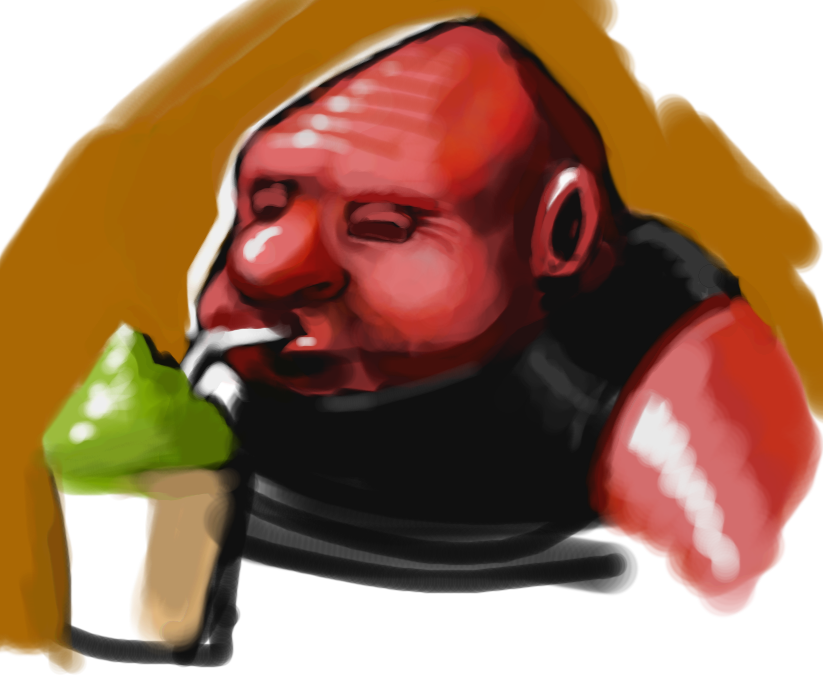
\includegraphics[width=0.45\textwidth]{images/paintings/brice2} }
		\subfloat[Homme avec puce sur un éléphant par \emph{Brice Vandemoortele}]{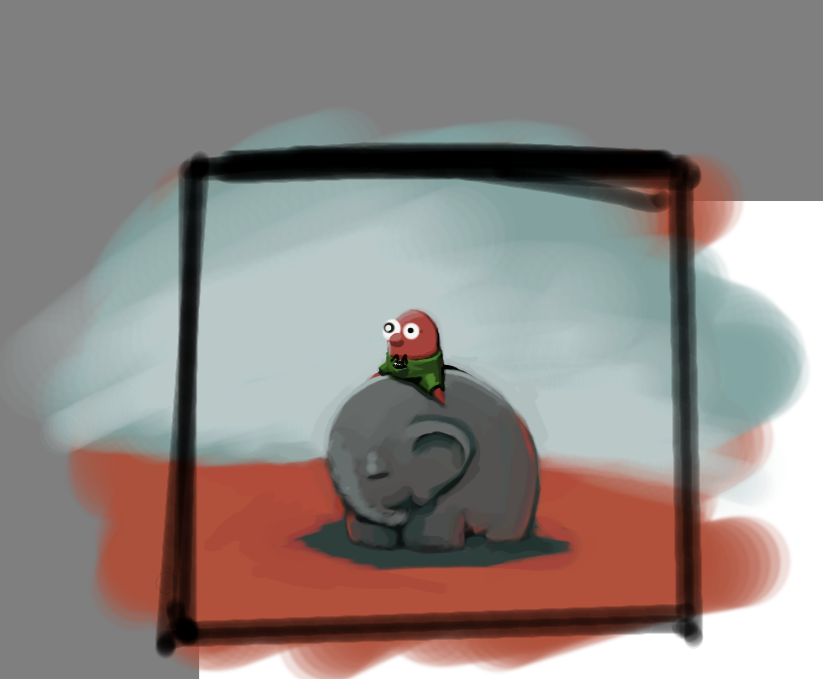
\includegraphics[width=0.45\textwidth]{images/paintings/brice3}}
		\\
		\subfloat[Homme avec puce sur un éléphant, détail. Par \emph{Brice Vandemoortele}]{
\includegraphics[width=0.9\textwidth]{images/paintings/brice3b}}
		\\
		\subfloat[Portrait couleur par \emph{Jean-Philippe Servais}]{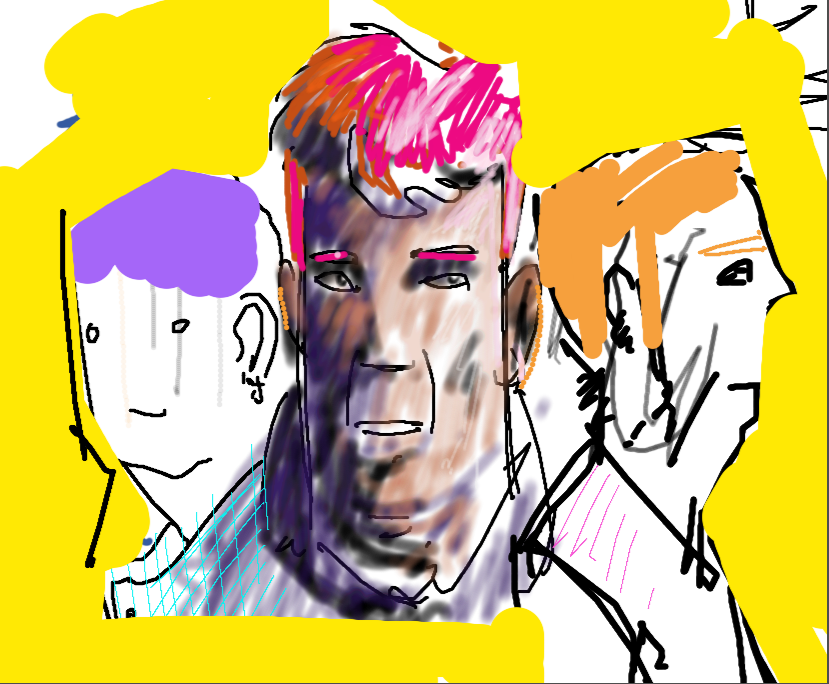
\includegraphics[width=0.45\textwidth]{images/paintings/jeanphi2} }
		\subfloat[Portrait au trait par \emph{Jean-Philippe Servais}]{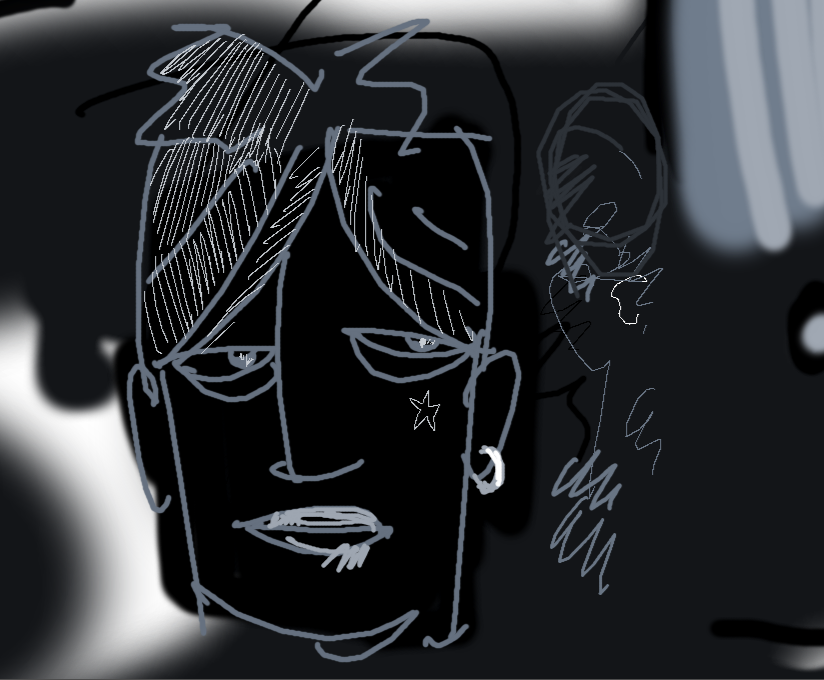
\includegraphics[width=0.45\textwidth]{images/paintings/jeanphi1} }
		\caption{Sélection de dessins terminés réalisés durant les tests}
		\label{fig:paintings}
	\end{figure}
	La figure~\ref{fig:paintings}, page~\pageref{fig:paintings} présente une sélection des dessins qui ont pu être terminés pendant les tests.
	
	L'annexe B, page~\pageref{annexb} présente l'intégralité des dessins réalisés par les utilisateurs durant ces tests. Notons que les sujets 
	imposés aux utilisateurs étaient parfois assez éloignés de leur spécialité. Il serait à ce titre intéressant de réaliser des tests plus libres
	qui laisseraient aux utilisateurs le choix de la méthode et du sujet. 
	
	\section{Analyse}
		\subsection{Performances de la peinture}
		Les performances de la peinture ont été jugées de correctes à excellentes dans tous les tests par tous les utilisateurs. Un utilisateur
		a justifié sa note de \emph{correct} au lieu de \emph{bien} par des ralentissements lorsque le rayon de la brush est grand par rapport
		à la région d'affichage en cours. Ceci est également mentionné lors des points négatifs. 
		Le problème n'est pas lié à l'algorithme de rasterisation et la seule manière de résoudre ce problème est 
		d'optimiser le code responsable du dessin de la primitive. Une autre solution est d'utiliser une machine plus performante; On notera
		que les testeurs sont habitués à travailler sur des machines nettement plus performantes que la machine dont ils
		disposaient pour le test. 

		On voit sur le graphe de performance, à la figure~\ref{fig:paintperf}, page~\pageref{fig:paintperf} que la plupart des mise à jour
		se fait dans des délais permettant l'interactivité. Le graphe (c) analyse de plus près les performances lors de la peinture. Les sauts
		de performances sont expliqués par des changements dans les paramètres de l'outil de peinture. Les raisons de l'évolution à la hausse
		des temps de rasterisation ne sont par contre pas encore claires. On trouvera à l'annexe A, page~\pageref{annexa} des graphes similaires
		pour l'intégralité des tests. 

		On observera également les grandes disparités qui existent entre les styles de peinture des utilisateurs, qui se traduisent par des
		différences significatives en terme de longueur et nombre de traits utilisés. Nous ne disposons cependant pas de suffisamment de
		données pour déterminer en quoi ces disparités influencent les performances. 

		\subsection{Déplacement de la région de visualisation}
		Cette fonctionnalité a également été jugée de correcte à excellente dans tous les tests par tous les utilisateurs. Ceux-ci n'ont pas
		eu de remarques particulières à énoncer à propos de cette fonctionnalité. Une analyse en détail des performances montre que le déplacement
		de la région de visualisation est généralement beaucoup moins fluide que la peinture. Le fait que ces deux fonctionnalités obtiennent des
		notes similaires témoigne que les utilisateurs ont des attentes de performances différentes pour chacune des fonctionnalités. 

		La plupart des temps de mise à jour de durées tournant autour de la seconde que l'on observe dans le graphe de performance correspondent
		à des déplacements particulièrement lents de la région de visualisation. 
		
		\subsection{Zoom/Dézoom}
		Le zoom/dézoom est la fonctionnalité qui a posé le plus de problèmes aux utilisateurs. Ses performances sont notées le plus souvent comme
		mauvaises ou inacceptables. En effet, le changement d'échelle est l'opération la plus lente, surtout l'agrandissement qui prend parfois
		jusqu'à plusieurs dizaines de secondes. Ces délais sont clairement visibles sur le graphe de performances. 
		
		Le problème est le suivant: La complexité de la rasterisation est en $O(n)$ ou $n$ est le nombre
		d'opérations affectant la région à visualiser ajoutées depuis la dernière rasterisation. 
		Lorsqu'un utilisateur peint au même endroit pendant une longue
		durée, et qu'il choisit de changer d'échelle, cette échelle n'aura pas été visualisée depuis longtemps, ce qui implique de 
		nombreuses opérations à recalculer. 
		
		Il y a plusieurs pistes pour améliorer le zoom. Par exemple, si une opération est opaque, les opérations précédentes ne sont pas exécutées,
		ce qui permet de réduire la complexité. Malheureusement, il est assez rare qu'une primitive masque complètement un tile. Cependant, les traits
		entiers couvrent régulièrement les tiles. Pour l'instant il n'est pas possible de s'en rendre compte à la rasterisation. Il serait cependant
		possible de faire cela si l'on implémentait la rasterisation de chaque trait dans une hlImage séparée, comme suggéré au chapitre sur l'anti-aliasing.
		En effet, l'opération de fusion est capable de détecter que l'image à fusionner (ici le trait) est opaque, et qu'il n'est pas nécessaire
		de connaître le résultat de l'opération précédente.

		En discutant avec les utilisateurs, on se rend compte, que le zoom est principalement utilisé comme moyen de visualiser ou de naviguer
		rapidement dans l'image à une échelle différente. Dans ces cas, la rapidité du zoom est plus importante que la qualité du rendu.
		Il serait donc possible d'afficher une approximation rapide de l'image à une échelle différente, et de mettre à jour cette approximation dès
		que l'on a rasterisé les tiles. Une approche similaire est utilisée avec succès par le Mégatexturing pour masquer la latence de l'accès aux 
		textures. 
		\subsection{Undo/Redo}
		Les notes données à l'undo/redo varient fortement entre les utilisateurs. Ces différences ne sont pas expliquées par une différence
		de performance à l'utilisation, mais par des attentes différentes des utilisateurs. Ainsi, l'un d'entre eux a systématiquement noté les performances
		comme \emph{mauvaises}  lorsque cette opération ne se réalisait pas instantanément, alors que d'autres utilisateurs semblaient très satisfaits
		de performances identiques. Le chapitre discutant de la gestion de la cache donne quelques pistes pour améliorer la performance 
		de l'undo/redo, qui pourraient permettre de satisfaire les demandes des utilisateurs les plus exigeants. 

		\subsection{Anti-Aliasing}
		L'anti-aliasing fut jugé de correct à excellent dans tous les tests par tous les utilisateurs. Des remarques particulières ont été émises,
		tant positives que négatives. La quantisation à faible opacité fut le problème principal. Une résolution de ce problème est
		proposée dans le chapitre sur l'anti-aliasing à la section \emph{Problème de fusion à faible opacité}, page~\pageref{fopac}. Un autre problème plus rare fut la disparition des traits à grande échelle. Ce problème est
		également expliqué dans la section \emph{Quantisation des très petites primitives}, à la page~\pageref{tpquan} du chapitre sur l'anti-aliasing.  Les utilisateurs ont cependant beaucoup apprécié l'aspect général du rendu, et 
		ont parfois qualifié l'anti-aliasing de meilleur que ce qu'ils utilisaient habituellement.  
		
\chapter{Conclusion}
	Ce mémoire nous aura donc permis d'explorer les principes de base du framework \emph{Himalaya} et 
	d'en identifier les principaux obstacles à son utilisation en tant qu'outil de peinture gigapixel.
	
	La plupart de ces problèmes furent résolus. Et pour chaque problème auquel nous n'avons pas pu apporter
	de solution définitive, nous avons pu identifier plusieurs pistes de résolution.

	Les tests utilisateurs nous ont permis de confirmer ce que la théorie laissait supposer;
	le framework que nous avons développé permet de peindre de manière interactive des images gigapixel en permettant
	aux utilisateurs de réaliser plusieurs peintures de résolution jusqu'alors jamais atteinte, tout en proposant une
	expérience satisfaisante. Si les tests ont révélé des lacunes de performances pour certaines fonctionnalités, 
	les discussions avec les utilisateurs ont permis d'identifier des pistes de résolution.


	Le chapitre sur l'utilisation du framework nous a également donné un aperçu de la facilité avec laquelle on peut 
	utiliser celui-ci pour réaliser des applications graphiques complexes. Les techniques présentées dans ce chapitre ont
	également été validées par l'implémentation d'une application utilisée pour les tests utilisateurs.

	Si les résultats expérimentaux sont positifs, les développements théoriques le sont aussi. Ceux-ci nous ont en effet 
	permis d'identifier un grand nombre de pistes qui devraient nous permettre d'améliorer encore de manière substantielle 
	les performances du framework :
	\begin{itemize}
		\item L'utilisation du multithreading.
		\item Une heuristique de cache globale
		\item Des migrations de la cache entre la mémoire vive et le disque dur.
		\item Des meilleures heuristiques pour les Bounding Opérations.
		\item Des améliorations au niveau de l'anti-aliasing.
	\end{itemize} 

	Outre ces possibilités, nous ne devons pas oublier certaines fonctionnalités dont nous avons parlé au premier chapitre qui
	n'ont pas été explorées dans ce mémoire. Nous pensons à la gestion des espaces colorimétriques, 
	aux transformations géométriques, aux filtres, à  l'intégration à un système de mégatextures ainsi qu'à la lecture et 
	l'enregistrement de fichiers. Il ne fait aucun doute que l'implémentation des ces dernières, et leurs
	tests pour des utilisations plus variées soulèveront de nouveaux problèmes méritant notre attention.


	%Il était une fois un homme. Seul, dans une ruelle étroite, il marchait, sans trop savoir ou aller. Perdu ? 
	%Certainement pas ! Il ne savait que trop bien ou il se trouvait ! Mais où aller ? Partout ou il promène ses
	%loques, partout ou il pose son regard las, il retrouve un endroit connu depuis une éternité... s'il y a bien
	%un endroit où l'on ne peut se perdre, c'est l'enfer.

	%L'enfer
	%. Une ville
	%ou tout se con


%	Les tests utilisateurs se sont vraiment avéré géniaux, les utilisateurs ont dansé, chanté et bu à
%	la gloire de mon programme, se sont protesté devant ses bugs, et imploré sa grâce divine. Cependant,
%	cela n'est qu'un début. Car en vérité je vous le dis, notre but va bien plus loin. Non! Nous ne nous
%	arrèterons pas au premier petit succès sans intérèt! Nous avancerons! Encore et toujours! Au delà des
%	limites du monde! Nous dépasserons les frontières de l'espace et du temps! Délaissant toute raison,
%	toute logique, et toutes basses considérations, nous ferons face à l'infini armé de notre seule foi dans
%	ce mémoire! Vous aussi, lecteur, abandonnez vous à l'univers et dépassez les limites. Ne mettez pas 18
%	là ou l'on pourrait mettre 19! Mettez 20! Mettez 21 ... Mettez 22 !
